\begin{figure}
\begin{center}
    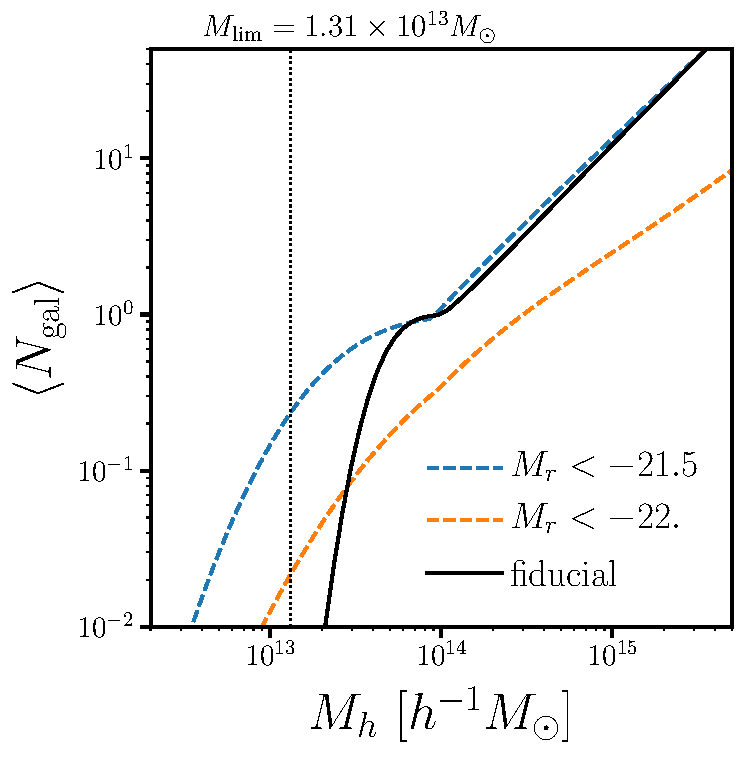
\includegraphics[width=0.45\textwidth]{figs/hod_fid.pdf} 
    \caption{Our fiducial halo occupation (black) parameterized using the
    standard \cite{zheng2007} HOD model. The parameter values of our fiducial
    HOD model (Eq.~\ref{eq:hod_fid}) are roughly based on by the best-fit HOD
    parameters of the SDSS $M_r < -21.5$ and $< -22.$ samples from
    \cite{zheng2007}, modified to accommodate the $M_{\rm lim}{=}1.31{\times}
    10^{13} h^{-1}M_\odot$ halo mass limit of the \quij~simulations (black
    dotted). We include the best-fit halo occupations of the SDSS  $M_r <
    -21.5$ (blue dashed) and $< -22.$ samples (orange dashed) from
    \cite{zheng2007} for reference. Since our HOD parameters are based on the
    high luminosity SDSS samples, we do not include assembly bias.  Our
    fiducial HOD galaxy catalog has a galaxy number density of 
    $\overline{n}_g \sim 1.63\times10^{-4}~h^3/{\rm Mpc}^3$ and linear bias of
    $b_g \sim 2.55$.
    }\label{fig:hod}
\end{center}
\end{figure}

\section{The Molino Mock Galaxy Catalogs: Halo Occupation Distribution} \label{sec:hod}  
We are interested in quantifying the information content of the galaxy bispectrum. 
For a perturbation theory approach, this involves incorporating an analytic bias model 
for galaxies~\citep[\emph{e.g.}][]{sefusatti2006, yankelevich2019, chudaykin2019}.
Perturbation theory approaches, however, break down on small scales and cannot
exploit the constraining power from the nonlinear regime. Instead, in our simulation-based 
approach, we use the halo occupation distribution (HOD) 
framework~\citep[\emph{e.g.}][]{benson2000, peacock2000, seljak2000,
scoccimarro2001a, berlind2002,
cooray2002, zheng2005, leauthaud2012, tinker2013, zentner2016, vakili2019}.
HOD models statistically populate galaxies in dark matter halos by specifying
the probability of a given halo hosting a certain number of galaxies. This 
statistical prescription for connecting galaxies to halos has been remarkably 
successful in reproducing the observed galaxy clustering and, as a result, is the standard approach for constructing 
simulated galaxy mock catalogs in galaxy clustering analyses to estimate covariance 
matrices and test systematic effects~\citep[\emph{e.g.}][]{rodriguez-torres2016, rodriguez-torres2017, beutler2017}. 
More importantly, HOD is the primary framework used in simulation-based galaxy
clustering analyses: \eg~emulation~\citep{mcclintock2018,
zhai2019} or evidence modeling~\citep{lange2019}. Since the forecasts we
present in this paper are aimed at quantifying the constraining power of the
galaxy bispectrum for simulation-based analyses, the HOD model is particularly 
well-suited for our purpose.

In HOD models, the probability of a given halo hosting $N$ galaxies of a
certain class is dictated by its halo mass --- $P(N|M_h)$. We use the standard
HOD model from \cite{zheng2007}, which specifies the mean number of galaxies in
a halo as
\beq
\langle N_{\rm gal} \rangle = \langle N_{\rm cen} \rangle + \langle N_{\rm sat} \rangle
\eeq
with mean central galaxy occupation
\beq \label{eq:Ncen}
\langle N_{\rm cen} \rangle  = \frac{1}{2}\Bigg[1 + {\rm erf}\bigg(\frac{\log M_h - \log M_{\rm min}}{\sigma_{\log M}}\bigg) \Bigg]
\eeq
and mean satellite galaxy occupation
\beq \label{eq:Nsat}
\langle N_{\rm sat} \rangle = \langle N_{\rm cen} \rangle \bigg(\frac{M_h - M_0}{M_1}\bigg)^\alpha.
\eeq
The mean number of centrals in a halo transitions smoothly from 0 to 1 for halos 
with mass $M_h > M_{\rm min}$. The width of the transition is dictated by 
$\sigma_{\log M}$, which reflects the scatter between stellar mass/luminosity and 
halo mass. For $M_h > M_{\rm min}$, $\langle N_{\rm sat} \rangle$ follows a power 
law with slope $\alpha$. $M_0$ 
is the halo mass cut-off for satellite occupation and $M_h = M_0 + M_1$ is 
the typical mass scale for halos to host one satellite galaxy. The numbers 
of centrals and satellites for each halo are drawn from Bernoulli and Poisson 
distribution, respectively. Central galaxies are placed at the center of the
halo while the position and velocity of the satellite galaxies are sampled from a 
\cite{navarro1997} (NFW) profile. 

For the fiducial parameters of our HOD model, we use the following values: 
\beq \label{eq:hod_fid}
\{\log M_{\rm min}, \sigma_{\log M}, \log M_0, \alpha, \log M_1 \} = \{13.65,~0.2,~14.0,~1.1,~14.0\}.
\eeq
These values are roughly based on the best-fit HOD parameters for the SDSS $M_r
< -21.5$ and $-22$ samples from \cite{zheng2007}. 
In Figure~\ref{fig:hod}, we present the halo occupation of our fiducial 
HOD parameters (black). We include the best-fit halo occupations of 
the SDSS $M_r < -21.5$ (blue)  and $-22$ (orange) samples from \cite{zheng2007}
for comparison. We also mark the  $M_{\rm lim}{=}3.2\times10^{13} h^{-1}M_\odot$ 
halo mass limit of the \quij~simulations (black dotted). At $M_h \sim 10^{13} M_\odot$, 
the best-fit halo occupations of the SDSS samples extend below $M_{\rm lim}$.
We, therefore, cannot use the exact best-fit HOD
parameter values from the literature and instead reduce $\sigma_{\log M}$ to 0.2 dex.
%As we mention above, $\sigma_{\log M}$ reflects the scatter between stellar mass/luminosity and halo mass. 
The high $\sigma_{\log M}$ in the $M_r < -21.5$ and $-22$ SDSS samples is
caused by the turnover in the stellar-to-halo mass relation at high stellar
masses~\citep{mandelbaum2006, conroy2007, more2011, leauthaud2012, tinker2013,
zu2015, hahn2019b}. Our fiducial halo occupation, with its lower $\sigma_{\log
M}$, reflects a galaxy sample with a tighter scatter between stellar
mass/luminosity and $M_h$ than the SDSS samples.  %than the samples selected based on $M_r$ or $M_*$ cuts, which were used in SDSS and BOSS. To
In practice, constructing such a sample would require selecting galaxies based on
observable properties that correlate more strongly with $M_h$ than 
luminosity or $M_*$. While there is evidence that such observables are 
available~\citep[\eg~$L_{\rm sat}$; ][]{alpaslan2019}, they have not been
adopted for selecting galaxy samples. Regardless, in this work
our focus is on quantifying the information content of the galaxy bispectrum 
and not on analyzing a specific observed galaxy sample. We, therefore, opt for 
a more conservative set of HOD parameters with respect to $M_{\rm lim}$, even
if the resulting galaxy sample is less reflective of observations. For our
fiducial halo occupation at the fiducial cosmology, the galaxy catalog has 
$\bar{n}_g \sim 1.63\times 10^{-4}~h^3~{\rm Mpc}^{-3}$ and linear bias of 
$b_g \sim 2.55$.
%We confirm using \quij simulations with higher mass resolution ($1024^3$ CDM particles) that $M_{\rm lim}$ does not impact the observables or their derivatives in our analysis for our fiducial HOD parameters. 

The halo occupation in the \cite{zheng2007} model depends solely on $M_h$. 
Simulations, however, find evidence that secondary halo properties such as
concentration or formation history correlate with the spatial distribution of
halos --- a phenomenon referred to as ``halo assembly bias''~\citep[\eg][]{sheth2004,
gao2005, harker2006, wechsler2006, dalal2008, wang2009, lacerna2014,
contreras2020, hadzhiyska2020}.
A model that only depends on $M_h$, does not account for this halo assembly 
bias and may not be sufficiently flexible in describing the connection between 
galaxies and halos. Moreover, if unaccounted for in the HOD model, and thus 
not marginalized over, halo assembly bias can impact the cosmological parameter constraints. 
However, for the high luminosity SDSS samples ($M_r < -21.5$  and $<-22$), 
\cite{zentner2016} and \cite{vakili2019} find little evidence for assembly bias 
in the galaxy clustering. Similarly, \cite{beltz-mohrmann2020} also find that
the \cite{zheng2007} HOD model is sufficient to reproduce galaxy clustering of
luminous galaxies in hydrodynamic simulations. Since we base our HOD parameters
on the high luminosity SDSS samples, we do not include assembly bias and use
the \cite{zheng2007} model. 


The \molino~suite of galaxy mock catalogs~\citep{hahn2020a} used in this paper 
are constructed using the $22,000$ $N$-body simulations of the \quij~suite: $15,000$ 
at the fiducial cosmology and $500$ at the 14 other cosmologies listed in Table~\ref{tab:sims}.
First, we construct mocks for estimating the
covariance matrices using the 15,000 \quij~simulations at the fiducial cosmology with
the fiducial HOD parameters. Next, we construct mocks for estimating the
derivatives with respect to cosmological parameters using the 500
\quij~simulations at each of the 14 non-fiducial cosmologies. Finally, we construct mocks for
estimating the derivatives with respect to the HOD parameters, using 500 
\quij~simulations at the fiducial cosmology with 10 sets of non-fiducial HOD
parameters --- a pair per parameter. Similar to the non-fiducial cosmologies in
\quij, for each pair we vary one HOD parameter above and below the fiducial
value by step sizes:
\beq
\{\Delta \log M_{\rm min}, \Delta \sigma_{\log M}, \Delta \log M_0, \Delta \alpha,
\Delta \log M_1 \} = \{0.05, 0.2, 0.2, 0.2, 0.2\}.
\eeq
These step sizes were chosen so that the derivatives are converged.
For the covariance matrix mocks, we generate one set of HOD realizations and apply 
RSD along the z-axis: 15,000 mocks. For the derivative mocks, we generate 5
sets of HOD realizations with different random seeds: 60,000 mocks. {\em In
total, we construct and use 75,000 galaxy catalogs in our analysis}.
The \molino~galaxy catalogs are publicly available at
\href{changhoonhahn.github.io/molino}{changhoonhahn.github.io/molino}.
